Tato diplomová práce demonstrovala, že pro vytvoření plnohodnotného \gls{plc}
systému je třeba zvládnou širokou škálu dílčích kroků. Od návrhu komunikačních
protokolů, přes návrh hardwaru, programování firmwaru, až po programování
počítačových aplikací a~knihoven. Autorovi se povedlo všechny tyto kroky
úspěšně zvládnout. Podařilo se mu vytvořit

\begin{compactitem}
\item nový master modul sběrnice \gls{mtbbus},
\item nový univerzální \textit{slave} modul sběrnice \gls{mtbbus},
\item nástavný modul do starších modulů \gls{mtbuni},
\item počítačovou aplikaci pro přístup k~systému \gls{mtb},
\item knihovnu pro integraci nového \gls{mtb} do současného řídicího systému
	kolejiště.
\end{compactitem}

Komponenty vytvořené v~rámci této práce a~jejich interakce jsou přehledně
zobrazeny v~\ref{fig:new-topology}.

\begin{figure}[ht]
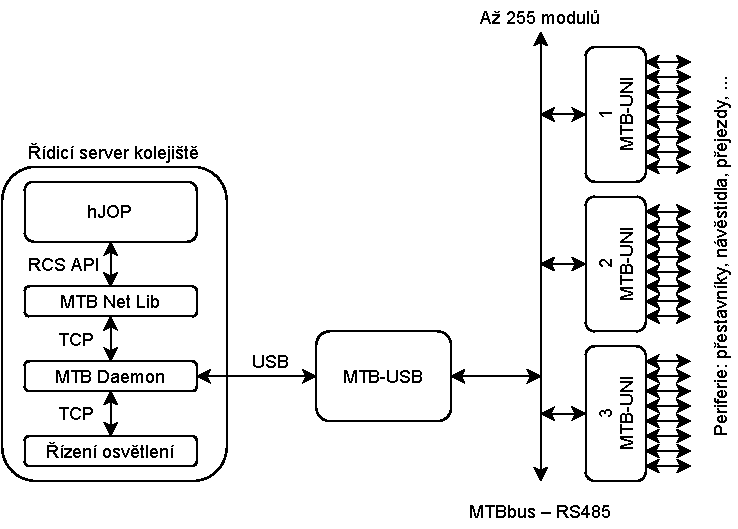
\includegraphics[width=0.8\textwidth]{data/new-topology.pdf}
\caption{Komponenty vytvořené v~rámci diplomové práce (mimo \textit{hJOP}).}
\label{fig:new-topology}
\end{figure}

V~rámci práce byly formulovány požadavky (\ref{sub:mtbbus-req-summary}), které
má nový systém \gls{mtb} splnit. Všechny tyto požadavky se podařilo naplnit.
Podařilo se vytvořit systém, který za poměrně malé finanční a časové náklady
značně povyšuje současný systém \gls{mtb}. Především však vznikl otevřený
a rozšiřitelný systém s~výhledem udržitelnosti po desítky let. Nový systém
\gls{mtb} umožní stavbu dalších kolejišť, udržování a rozšiřování kolejišť
současných. Nový systém \gls{mtb} si může vyrobit každý, kdo bude chtít bezpečně
řídit své modelové kolejiště.

V~termín odevzdání této práce je nový systém \gls{mtb} nasazen v~testovací
stanici o~4 \gls{mtb} modulech. V~termín obhajoby této práce se očekává nasazení
systému na kolejišti o~20 \gls{mtb} modulech. Přes léto roku 2021 se očekává
nasazení \gls{mtb} na největším kolejišti v~\gls{kmz} o~70 \gls{mtb} modulech.

\section{Možná rozšíření} \label{sec:future}

Při návrhu tak velkého systému, jako je \gls{mtb}, se přirozeně ukázaly mnohé
cesty, které by bylo možné v~budoucnu prozkoumat.

Systém \gls{mtb} by v~budoucnu mohl podporovat vyšší rychlosti komunikace nebo
automatickou detekci rychlosti sběrnice. \gls{mtb} by mohlo být rozšířeno
o~jednotky, které provádějí retranslaci dat sběrnice bezdrátově (pro vzdálené
připojení modulů).

Jednou z~otázek týkajících se budoucího rozšíření je, jak umožnit, aby systém
\gls{mtb} mohl interagovat s~komerčními softwary pro řízení modelových
kolejišť. Systém \gls{mtb} je navržen tak, aby takovou interakci umožnil.
Dalším možným rozšířením je tak implementovat do majoritních komerčních
softwarů pro řízení modelových kolejišť podporu pro \gls{mtb}. Některé softwary
jsou však uzavřené. Pro takové softwary by bylo možné napsat alternativní
firmware do \gls{mtbusb} desky, který by zajistil, že \gls{mtbusb} modul se pro
počítač bude tvářit jako některý z~komerčních systémů pro řízení kolejišť.

Dalším přirozeným způsobem rozšíření, který autor této práce má v~plánu
v~nejbližším roce uskutečnit, je přidání dalších typů modulů. V~budoucnu
vzniknou \gls{mtb} moduly pro chytré zesilovače \gls{dcc} signálu,
\textit{RailCom} detektory a jiné. Systém \gls{mtb} je na tato rozšíření
připraven.
